The implementation, integration and testing of the system will be perfomed following mainly a bottom-up approach, with some exceptions due to the complex system architecture.
Given the microservices architecture, lower-level services will be implemented and tested first, and then gradually integrated with higher-level components.
This approach is preferred because it allows to test the system as soon as possible, and to identify and fix bugs early in the development process, reducing the need of implementing complex stubs.
External services do not need to be tested, as it is assumed that they are already tested and reliable.
The testing will be performed in parallel with the implementation, and will be carried at different levels: unit testing, integration testing and system testing.
Regression testing will be performed at each level, to ensure that new changes do not break existing functionalities.
Also user acceptance testing is considered, to ensure that the final system meets the requirements of the customer.

\subsection{Plan}
In the first step, components that do not rely on others will be implemented and tested. These are the ServiceRegistry, EventQueue, NotificationQueue and SubmissionQueue components.
Note that, even if the queues are not depending on other components, to be tested it is needed to simulate the services that will consume them. For this reason, stubs of the EventService, NotificationService and SubmissionService will be needed.
Given the fact that ServiceRegistry covers a fundamental role in the synchronous communication between services, it will be implemented and tested before the other service components. 
However, in the following pictures, the connection between ServiceRegistry and other services is not shown, to avoid cluttering the diagrams.
\begin{figure}[H]
    \centering
    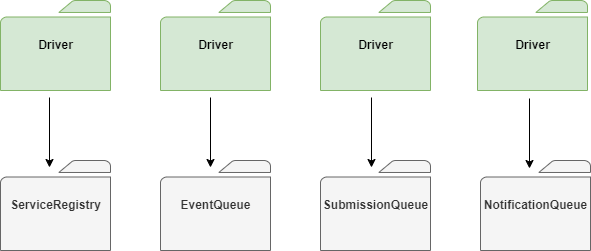
\includegraphics[width=0.6\textwidth]{Diagrams/integration_1.png}
    \caption{Bottom-up step 1}
\end{figure}

As second step, components that depends on the previous ones and on external services will be implemented, tested and integrated. These are the NotificationService and the GitHubIntegrationService.
The NotificationService consumes the NotificationQueue, so it replaces the corresponding stub. For this reason, the previous driver introduced to test the NotificationQueue can be reused.
\begin{figure}[H]
    \centering
    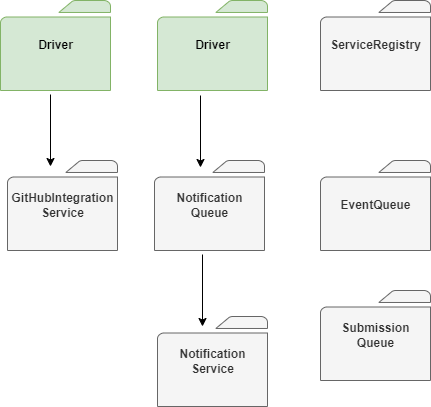
\includegraphics[width=0.5\textwidth]{Diagrams/integration_2.png}
    \caption{Bottom-up step 2}
\end{figure}

The third step will introduce in the systems two fundamental services: the TournamentService and the AuthService. Being both composed of two subcomponents (managers and models), they also should be implemented and tested incrementally:
starting the implementation from models, no stubs will be needed to test managers, and then the two subcomponents will be integrated together.
However, since the TournamentService relies on the EventService as event consumer, a stub of the EventService will be needed to test the TournamentService.
\begin{figure}[H]
    \centering
    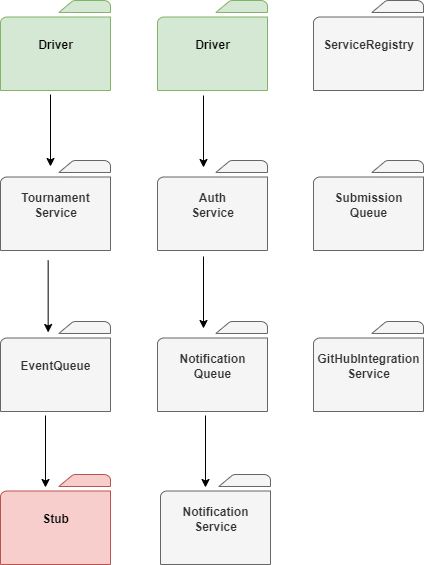
\includegraphics[width=0.5\textwidth]{Diagrams/integration_3.png}
    \caption{Bottom-up step 3}
\end{figure}

The fourth step includes the implementation of the EventService and EvaluationService.
\begin{figure}[H]
    \centering
    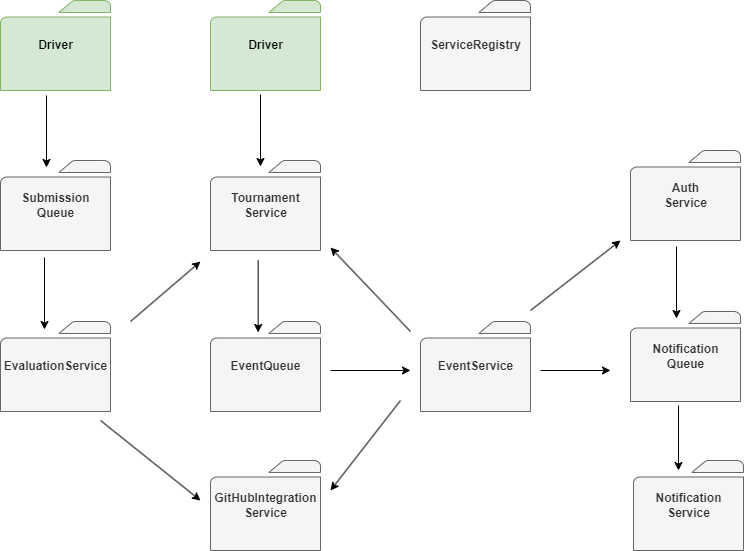
\includegraphics[width=0.8\textwidth]{Diagrams/integration_4.png}
    \caption{Bottom-up step 4}
\end{figure}

As fifth step, the APIGateway is implemented and integrated with the rest of the system. To test the APIGateway, a driver is needed. In particular, this driver, in addition to simulating the web calls related to the webapp, will also need to simulate the external calls of the GitHubActions service.
\begin{figure}[H]
    \centering
    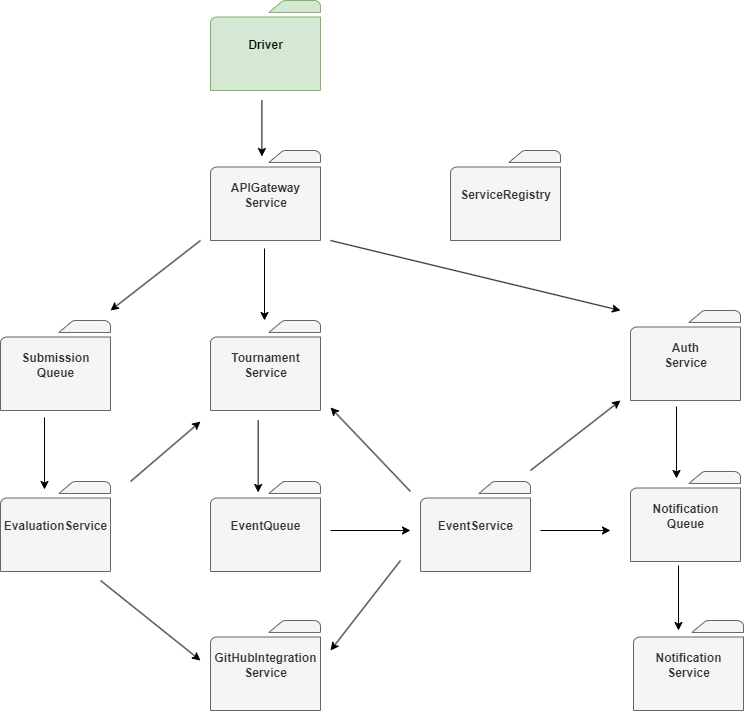
\includegraphics[width=0.8\textwidth]{Diagrams/integration_5.png}
    \caption{Bottom-up step 5}
\end{figure}

Finally, the WebApplication is implemented and tested, concluding the implementation and integration of the whole system.
\begin{figure}[H]
    \centering
    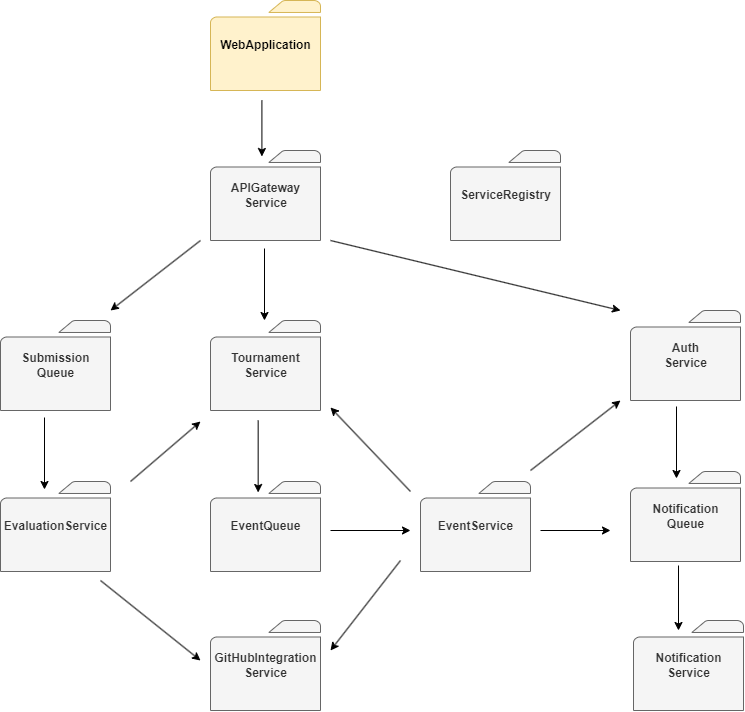
\includegraphics[width=0.8\textwidth]{Diagrams/integration_6.png}
    \caption{Bottom-up step 6}
\end{figure}

\subsection{E2E Testing}

Once the system is fully integrated, Selenium will be adopted as main framework for automating end-to-end testing of the web application, covering multiple browsers to ensure optimal compatibility.
Tests will simulate real user workflows that have been identified in the RASD. Each workflow such as signup, creation of a tournament, battle enrollment, etc. will be scripted to replicate user actions, data entry, navigation between pages, and validation of responses.
Assertions will be written to verify expected UI updates, error messages, database changes, and integration with external services. Tests will be data-driven to cover different use cases and scenarios.
